\documentclass[hidelinks,12pt]{report} % ---- COMPILE WITH XeLaTeX for Unicode!!! ----
\usepackage[a4paper, top=1in, bottom=1in, left=1.5in, right=1in]{geometry} % Set margins
\usepackage{setspace} % allows \doublespacing & \singlespacing
\usepackage{parskip} % enables non-indented paragraphs with a blank line
\usepackage[labelfont=bf]{caption}

% enables graphics, all figures and images should be in the /figures/ folder:
\usepackage{graphicx}
\graphicspath{{figures/}}

% enhanced maths symbols and syntax:
\usepackage{amsmath}
\usepackage{amssymb}
%\usepackage{amsthm} % if you need mathematical definitions and theorems

\usepackage[ruled]{algorithm2e} % allow for algorithms in pseudocode
\usepackage{listings} % allow for source code algorithms/listings
\lstset{basicstyle=\footnotesize, frame=single, numbers=left} % customise listing style

% Customise chapter headings so they are of the format: 1. Introduction
\usepackage{titlesec}
\titleformat{\chapter}[block]
  {\normalfont\huge\bfseries}{\thechapter.}{1em}{\Huge}
\titlespacing*{\chapter}{0pt}{-20pt}{20pt}

% Setup bibliography - add file to project named bibliography.bib
% can create this from Zotero, Mendeley, refworks, etc
\usepackage[numbers]{natbib}
\bibliographystyle{IEEEtranN}
%\setcitestyle{authoryear,open={(},close={)}, aysep={,}}

\usepackage{hyperref} % add links to document

\usepackage{url} % cite urls

\doublespacing
\begin{document}

\pagenumbering{roman} % Roman numeral page numbering up to the first page of introduction
\setcounter{page}{3} % Start at "ii", to count title page as "i"

\chapter*{Abstract} % \chapter* means the chapter is not in the contents or numbered
\addcontentsline{toc}{chapter}{\numberline{}Abstract}%
Microphone arrays have become increasingly popular due to their usefulness in a variety of speech related applications. A lot of studies have been conducted on microphone arrays, with commercial products such as Amazon Echo enjoying widespread usage.

However, existing commercial microphone array systems are either not easily customizable, difficult to deploy or too costly to be used in microphone array research and development. Thus, this project aims to develop a microphone array system that is both overcomes these issues while still being robust enough to handle heavy usage.

This project uses MATRIX Creator alongside Raspberry Pi as the hardware of choice due to their ease of deployment, customization, and their relatively small size. A mobile application was developed in tandem with this system to provide a wireless architecture. WiFi tethering is used to form an ad-hoc network of any number of microphone array devices that can operate synchronously for real world applications and provides a method to upload saved data to a cloud server via cellular network.

To ensure that the system is robust enough to handle heavy usage, wake word detection is used to conserve computational power and power consumption. The system also introduces Voice Activity Detection (VAD) to only save voiced data and discard the remaining data to conserve memory storage.  
The battery-life of the system can last up to 100 hours in passive-listening mode and up to 30 hours of active recording usage which is sufficient for practical applications. 

Audio samples were tested to ensure the best sample accuracy between devices and the results showed a sample deviation of around 30 samples, showing a large improvement over the non-synchronized version which has a sample deviation of around 500 samples.
Overall, the developed system has met the objectives of being easy to customize and deploy while still meeting real-world use case requirements. Therefore, this project could potentially bridge the gap between developers and end-users while helping to facilitate future research and development on microphone arrays.


\chapter*{Acknowledgements}
\addcontentsline{toc}{chapter}{\numberline{}Acknowledgements}%
This Final Year Project was made possible thanks to the constant support from various people. They have my utmost gratitude. 

Firstly, I would like to thank my supervisor, Associate Professor Chng Eng Siong, for the guidance, confidence, and opportunities that he has shown me. Dr Chng has helped me to see the potential in my project and has inspired me to constantly improve my project. 

I would also like to thank all the supportive staff and personnel at the Multimedia and Interactive Computing Lab at Nanyang Technological University. I would especially like to thank Zin and Ms. Ho for their assistance in guiding me regarding logistics and administration matters. 

I also want to acknowledge Professor Xiong Hu and his team in assisting me to further explore various aspects of this project with a renewed perspective. 

Finally, I would like to thank my friends and family for their encouragement during the stressful periods of this project. I would like to thank Ms. Andrea Jane for her advise in report writing and Ms. Tamara Edwina for her guidance and technical knowledge.  


\tableofcontents

\listoffigures
\addcontentsline{toc}{chapter}{\numberline{}List Of Figures}%

\listoftables
\addcontentsline{toc}{chapter}{\numberline{}List Of Tables}%

\chapter{Introduction}
\pagenumbering{arabic} % Introduction starts at page 1.




\section{Background}

Microphone arrays are devices that use multiple microphones operating together to record sound as opposed to only using one microphone. Microphone arrays that have been properly configured have been shown to greatly increase the quality of speech in audio recordings and therefore have found a great number of applications in the field of speech recognition\cite{1}. The popularity of products such as Amazon Echo and Google Nest are examples of the wide-ranging applications of microphone arrays. 

One noteworthy application of microphone arrays is their use in recording of meetings and conferences. Research has shown that microphone arrays are able to produce high quality replication of the spatial information of the environment\cite{2}. High quality recordings of meetings and conferences with microphone arrays can also improve the performance of speaker identification algorithms\cite{3}.

However, many of the current systems of meeting transcriptions involve microphone arrays that are either difficult to deploy due to either physical size, requiring installation, lack of customizability, or are too costly. Furthermore, many of the current microphone array devices do not have any form of interface for easy testing and development. This presents a challenge for further research and development of microphone array systems.

To overcome these problems, the Raspberry Pi and MATRIX Creator were chosen as the hardware to support this system. Due to their relatively small size and ease of customization, these devices were found to be the most suitable for this system. A further analysis of possible alternative devices and their comparisons can be found in the Literature Review chapter of this report. 

Finally, due to the devices not having any form of customizable user interface for testing, a mobile application was chosen as the most suitable option. This is because mobile devices are widely adopted, portable and support a wide range of communication protocols to interface with other hardware devices. To streamline the development, the cross-platform framework Flutter will be used to develop the mobile application.

\section{Objectives}

The main objective in this project is to develop a microphone array system that is both easily customizable and deployable in real world environments such as conference meetings, with minimal setup and configurations. The system should also be able to support development and testing of speech related algorithms. The system must achieve this while being able to handle long usage in terms of both memory storage and power consumption to be reliable and robust.

To achieve these the following functionalities are proposed for the system:

	\begin{itemize}
	\item{\textbf{Mobile cross-platform application as Master Controller}}\linebreak
	The mobile application will act as the interface for the user to issue a variety of commands to the system. These include adding or removing devices from the ad-hoc network, setting of various recording parameters, and uploading files to a cloud server.

	\item{\textbf{Wake word and Synchronized Voice Activity Detection}}\linebreak
	To save power and memory while not actively recording, the device will wait for a specified “wake word” before starting computationally heavy tasks such as initiating connections and recording. Similarly, to save memory usage, the device will have Voice Activity Detection functionality to only save audio data when speech 		has been detected and discard all other non-voiced data. 

	\item{\textbf{Synchronized Multi-device Multichannel Recording}}\linebreak
	As devices are added to the ad-hoc network, these devices will need to be synchronized to ensure that all devices being recording at the same time. As the individual microphones on each microphone array should already synchronized at the hardware level, synchronization will only need to be performed among different devices. 
	\end{itemize}
\section{Scope}

This report will cover only implementation specific to the Raspberry Pi, MATRIX Creator and Flutter applications. Furthermore, the Flutter aspect of the code is currently only tested with iOS devices. However, the source code for the Raspberry Pi and MATRIX Creator can also be extended to the MATRIX Voice. 

Furthermore, this project consists of two different versions, one version for use with a mobile device and another for use with a regular laptop or computer. Only the mobile version shall be discussed in this report as the other version is maintained solely for easy testing and debugging. 

\section{Report Organization}

This report is divided into six chapters, the overview of each section is described below:

	\begin{itemize}
	\item{Chapter 1 describes the introduction of the project, the motivation behind the project and the scope of the project.}
	\item{Chapter 2 explores the various literatures of related works that are used in this project.}
	\item{Chapter 3 provides an overview of the proposed microphone array system along with the concepts and ideas used in the design of this system.}
	\item{Chapter 4 describes in detail the implementation of the proposed system.}
	\item{Chapter 5 elaborates on the testing methods used along with a description and evaluation of the test results.}
	\item{Chapter 6 concludes the report and summarizes the problems faced and future suggestions in developing the microphone array system.}
	\end{itemize}




\chapter{Literature Review}

In this chapter, we will explore the existing literatures on topics related to the development of this project. This includes microphone arrays and their corresponding technologies and applications. We will also explore some important technologies related to the development of a microphone array system. Finally, we will compare the related products and technology frameworks that are useful for the design of the microphone array system. 

\section{Microphone Array}

A microphone array is defined as any number of microphones operating in tandem. They can be designed to have as many microphones as needed to record sound. Microphone arrays can also come in a variety of geometric structures, some examples of these structures are listed below.

\begin{figure}[h]
\centering
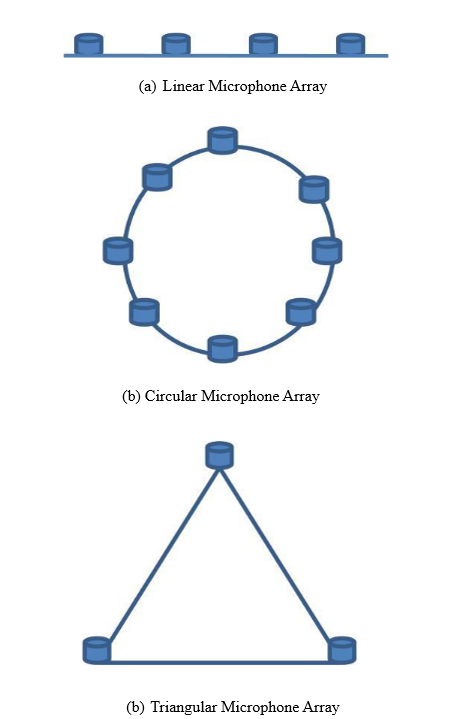
\includegraphics[scale = 1.0]{fig2.1} 
\caption{Various Microphone Array Configurations}
\label{fig}
\end{figure}


Microphone arrays have enjoyed widespread usage in speech related research due to their advantages over singular microphones. This includes the ability to capture the spatial features of the speech signal and reducing the signal to noise ratio\cite{4}.    

\section{Microphone Array Technologies}

This section covers the common technologies used in tandem with microphone arrays, namely, beamforming and direction of arrival. 

\subsection{Direction Of Arrival}

Beamforming is a signal processing technique that aims to increase the strength of the desired signal by means of controlling the phase and relative amplitude of the signal at the transmitter or receiver array\cite{5}. 

One common method of beamforming is known as the delay-and-sum beamformer. Given a known direction of arrival of the incoming signal, the beamformer sums the delayed signals arriving at the microphone array. This causes destructive interference of signals coming from all direction except for the original direction of arrival, thus enhancing the relative signal strength of the desired signal\cite{6}. 

Another method known as adaptive beamforming or null-steering beamforming improves upon the precious delay-and-sum beamformer. The adaptive beamformer system seeks to maximize or minimize a desired parameter such as signal-to-interference-plus-noise ratio in order to maximize gain of the desired signal\cite{7}.

Beamforming can be used in tandem with microphone arrays to solve a multitude of problems. One study conducted showed how beamforming was used to increase the ability of people with hearing loss to identify unique speakers in a crosstalk speaking environment\cite{8}.


\subsection{Beamforming}

In signal processing, direction of arrival refers to the direction at which the propagating wave arrives at a point. This direction is useful in many applications of speech processing such as acoustic source localization\cite{9} and beamforming as described in the previous section. 

One such algorithm to estimate the direction of arrival of a signal is the Estimation of Signal Parameters via Rotational Invariant Techniques (ESPRIT) algorithm. This algorithm uses the eigenvalue decomposition of subarrays from the covariant matrix of the complete microphone array to calculate the most likely direction of arrival. The estimation can be further improved by increasing the number of sensors or microphones in the sensor array\cite{10}.

Multiple Signal Classification (MUSIC) is another similar algorithm that also uses eigenvalue decomposition of the covariance matrix of the microphone array to estimate direction of arrival\cite{11}.

Studies have found MUSIC to produce a more precise direction of arrival as compared to ESPIRIT. However, the MUSIC algorithm is more complex and thus requires more computation overhead as compared to ESPIRIT\cite{12}.


\section{Synchronization Algorithms}

Since most audio array processing algorithms assume that the locations of sound sources have unique time differences of arrival in relation to the microphone array, even a small variance in sample synchronicity between microphones can result in drastically inaccurate performance\cite{13}. This section discusses two commonly used protocol for synchronizing devices. 

\subsection{Network Time Protocol}

\begin{figure}[h]
\centering
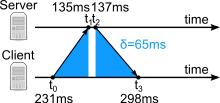
\includegraphics[scale = 1.0]{fig2.2} 
\caption{Visual Diagram of Network Time Protocol}
\label{fig}
\end{figure}

Network Time Protocol (NTP) is a protocol designed by David L. Mills in 1985 to synchronize devices to a theoretical millisecond accuracy. This protocol achieves synchronization by having a NTP client poll multiple NTP servers. This client then calculates its offset from the server clock and then adjusts its own clock. To increase the accuracy of the synchronization, the client repeats this process with multiple servers and any offset data that is deemed to be statistical outliers are discarded\cite{14}. 

\subsection{Precision Time Protocol}

Precision Time Protocol (PTP) is an extension of the traditional NTP that is intended to be used in local area networks where accuracies not attainable via the use of the regular NTP. 

A master device is first designated in the network and all slave devices perform synchronization with respect to the master device. The slave first sends a sync request message to the master and the master then responds with a sync response message. All messages are timestamped. This is followed by a delay request and delay response message between the slave and the master. 

By using the timestamp information, the slave can calculate its offset from the master clock and adjust itself accordingly. This process is then repeated, and the offset results averaged to accommodate for delays in network traffic or packet loss. PTP can potentially achieve sub-microsecond precision\cite{15}.

\section{Speech-based Technology Applications}

This section covers the common applications of speech related signal processing. The described applications could be potential features of the developed microphone array system.

\subsection{Voice Activity Detection}

Voice Activity Detection (VAD) is a speech processing technique to detect the presence or absence of human voice. As most speech processing algorithms perform poorly in the presence of noise or unwanted signals, VAD is commonly used to first filter out the speech signals for further processing. This can also reduce computational and memory overhead by disabling certain features of the speech processing when no speech activity is detected\cite{16}.

VAD has also become increasingly popular in applications where hands-free interaction is required\cite{17}. Thus, VAD could be useful in applications where either long period of usage is expected or accessibility to the microphone array device is limited.

\subsection{Hot Word}

Hot word or key word detection is a popular speech processing technique to identify certain key phrases in utterances. Like VAD, this method can reduce computational and memory overhead by disabling certain computationally heavy features when not in use. 

Since the aim of most hot word detection systems are to reduce computational overhead, the design of the detection system itself must be light-weight and have low latency. Research has shown that the usage of multiple microphones might provide increased performance and accuracy of a hot word detection system\cite{18}.

\section{Devices with Microphone Arrays}

This section explores some of the commercially available microphone array products including both end-user products and prototyping products. The products will then be compared to assess their suitability to be used in this project. 

\subsection{Commercial Systems with Microphone Array}

This section outlines a few of the more popular commercial microphone systems and their capabilities.

\subsubsection{Sony MAS-A100 Beamforming Microphone}

\begin{figure}[h]
\centering
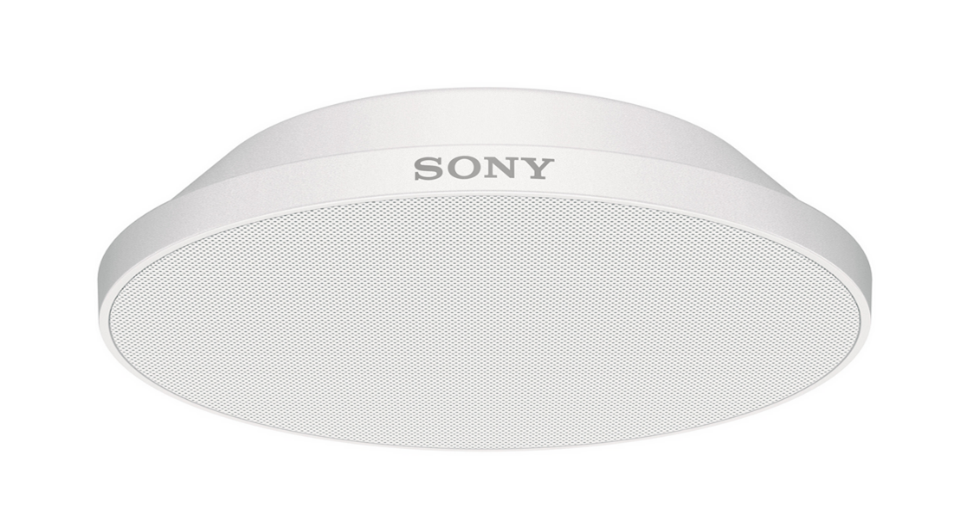
\includegraphics[scale = 1.0]{fig2.3} 
\caption{Sony MAS-A1000 Beamforming Microphone}
\label{fig}
\end{figure}

The Sony MAS-A100 microphone is a two channel microphone that is meant to be attached to the ceiling of a room in order to provide automatic recording. It features a multitude of audio related technologies such as noise reduction and beamforming. It also features an application programming interface for customization.

However, the MAS-A100 microphone requires a cabled connection and is costly and time-consuming to setup and thus might not be suitable for an easy to deploy system\cite{19}.

\subsubsection{Roland R-88 Multichannel Recorder}

\begin{figure}[h]
\centering
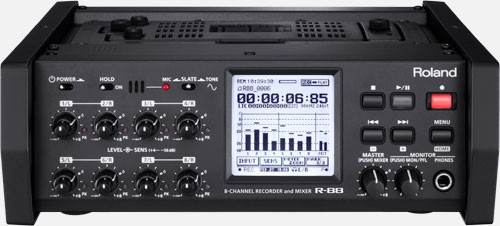
\includegraphics[scale = 1.0]{fig2.4} 
\caption{Roland R-88 Multichannel Recorder}
\label{fig}
\end{figure}

The Roland R-88 Multichannel Recorder is an interface that allows synchronized recording of up to 8 microphones. It also features customizable sampling rate, removable SD card system and a 3-band equalizer.

However, due to the bulky nature of the product, need for external microphones and the need for an external cabled power supply, this product is deemed not portable enough for the proposed microphone array system\cite{20}. 

\subsubsection{Amazon Echo}

\begin{figure}[h]
\centering
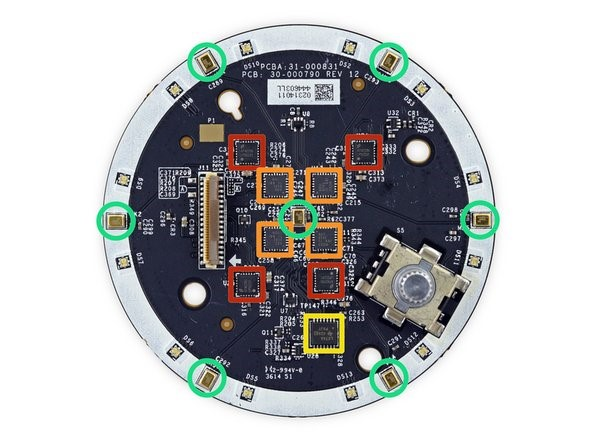
\includegraphics[scale = 0.5]{fig2.5} 
\caption{Cross Section View of the Amazon Echo's Microphone Array}
\label{fig}
\end{figure}

The Amazon Echo is a smart-home automation device that features a microphone array for hands-free operation. It features WiFi and Bluetooth connectivity, a partner application as well as Amazon’s Smart Home Skill API for further customization. 

However, while the API provides a decent amount of control over the Amazon Echo’s hardware, the microphones are not customizable. This could hinder any further microphone array research\cite{21}.

\subsection{Development Boards with Microphone Array}

This section outlines the available development boards that have microphone array functionalities. It also describes the other features that are available in these hardware devices.

\subsubsection{UMA-8 Microphone Array}

\begin{figure}[h]
\centering
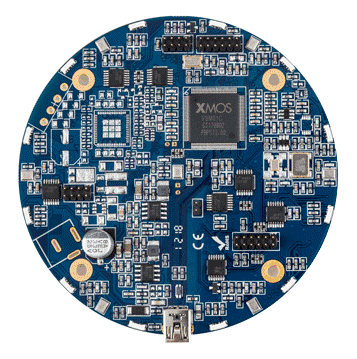
\includegraphics[scale = 1.0]{fig2.6} 
\caption{UMA-8 Microphone Array}
\label{fig}
\end{figure}

The UMA-8 Microphone Array is a circular microphone array that is designed to be connected to any Linux/Mac/Windows device via USB. It has pre-built firmware that includes beamforming, direction of arrival and noise cancellation.

However, the UMA-8 does not provide any application programming interface for easy customization and only provides limited shell-script programming options. This could limit testing of any potential speech-related algorithms that are not built into the existing firmware\cite{22}. 

\subsubsection{Respeaker 6 Mic Array for Pi}

\begin{figure}[h]
\centering
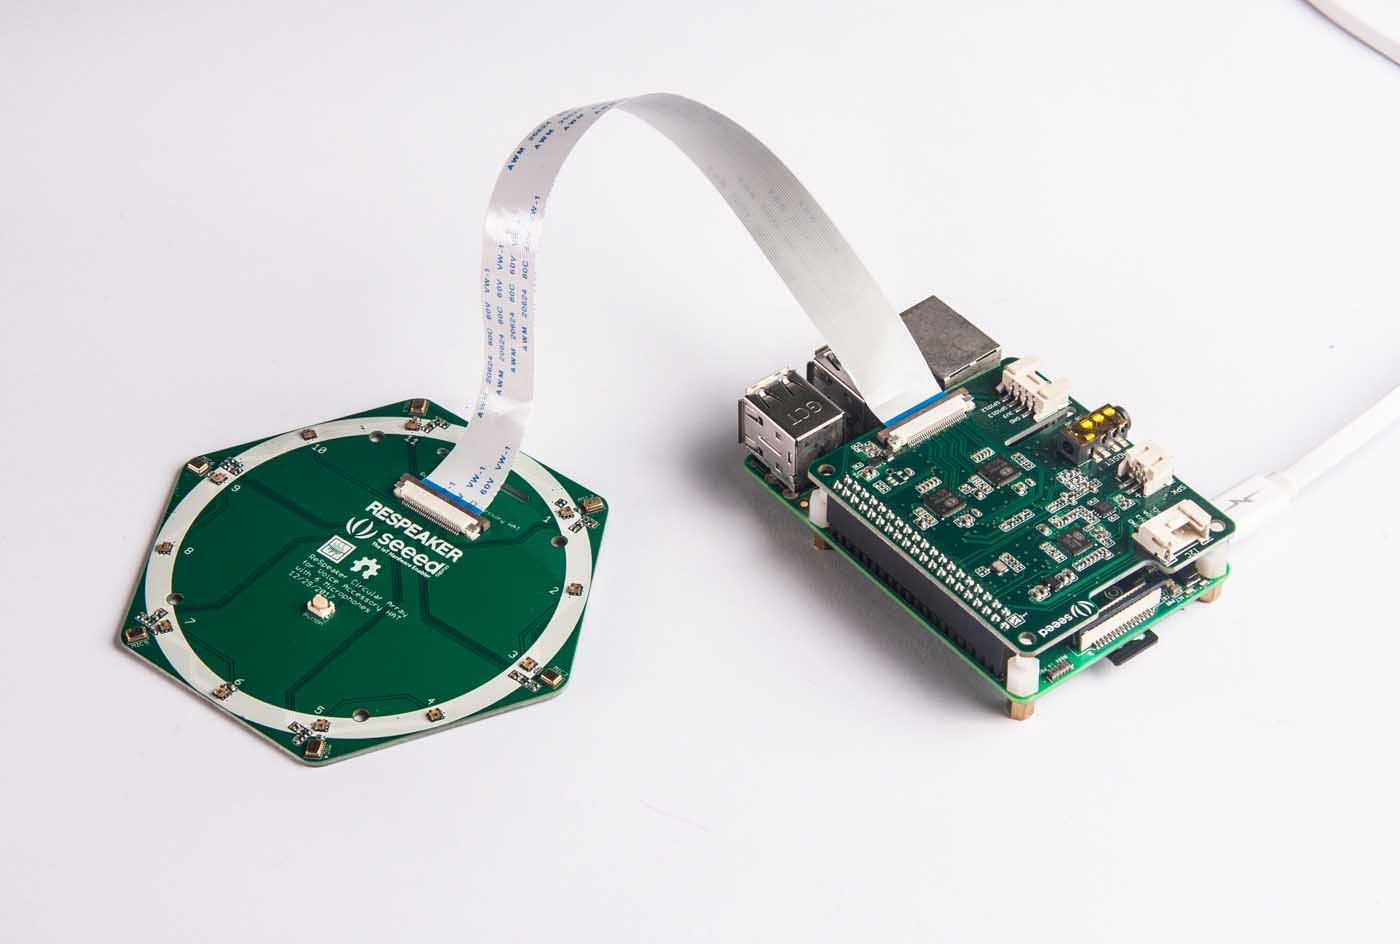
\includegraphics[scale = 1.0]{fig2.7} 
\caption{Respeaker 6 Mic Array connected to a Raspberry Pi}
\label{fig}
\end{figure}

The Respeaker 6 Mic Array is designed to be used with the Raspberry Pi via the Pi’s GPIO pins. It features 6 MEMS microphones and provides software development kits for C++ and Python\cite{23}. 

\subsubsection{MATRIX Creator}

\begin{figure}[h]
\centering
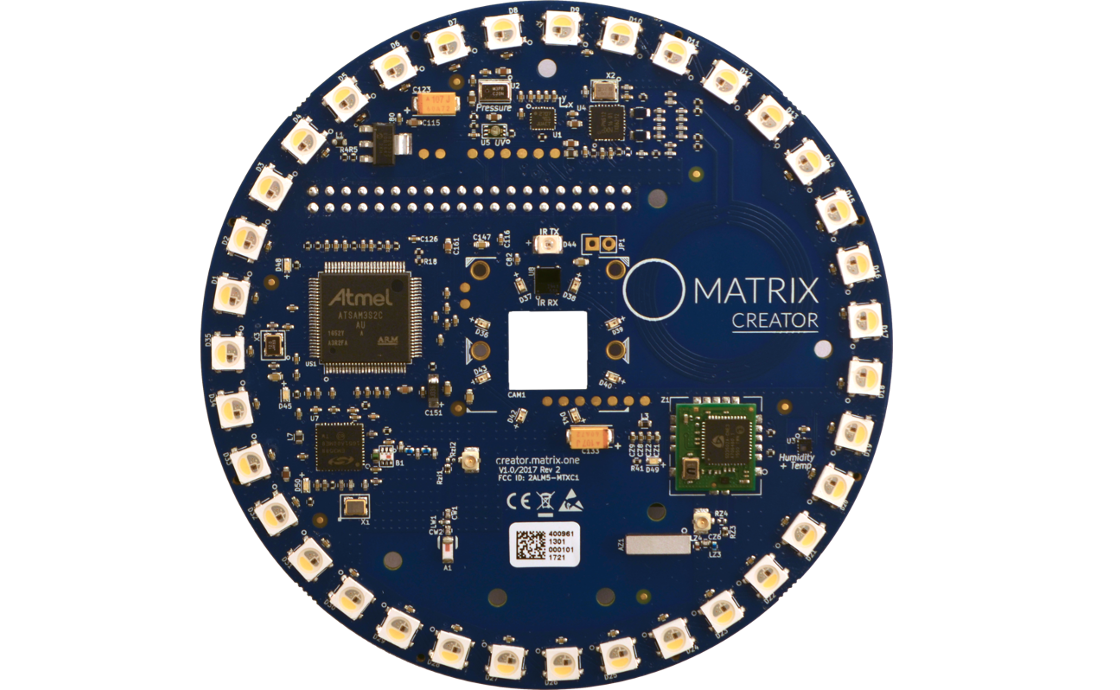
\includegraphics[scale = 0.2]{fig2.8} 
\caption{Top View of the MATRIX Creator}
\label{fig}
\end{figure}

The MATRIX Creator is another circular microphone array that is designed to be used with the Raspberry Pi via its GPIO pins. It features 8 MEMS microphones and various libraries and software development kits for easy customization with Python, Java and C++. 

As the MATRIX Creator is designed as an IoT prototyping tool, it also provides many other features such as humidity sensor, IR receiver and transmitter, ZigBee and NFC. A full listing of the MATRIX Creator’s features can be found in Appendix A.

\subsection{Comparison of Microphone Array Devices}



\begin{table}[]
\begin{center}
\scalebox{0.9}{
\begin{tabular}{|l|l|l|l|l|l|}
\hline
\textbf{Product} & \textbf{Cost(USD)} & \textbf{Portable} & \textbf{Cuztomizable} & \textbf{Ch} & \textbf{Sample Rate(kHz)} \\ \hline
MAS-A100         & 2,146              & No                & No                    & 2                           & 48                           \\ \hline
Roland 88        & 968.13             & No                & No                    & 8                           & 44.1/48/88.2/96              \\ \hline
Amazon Echo      & 63.70              & Limited           & Limited               & 6                           & 44.1/48                      \\ \hline
UMA-8            & 95+36              & Yes               & Limited               & 8                           & 11.2/16/32/44.1/48           \\ \hline
Respeaker 6      & 58+36              & Yes               & Yes                   & 6                           & 8/16/44.1/48                 \\ \hline
MATRIX Creator   & 102+36             & Yes               & Yes                   & 8                           & 8/16/44.1/48/88.2/96         \\ \hline
\end{tabular}}
\label{tab:tablelabel}
\caption{Comparison of various Microphone Array Devices}
\end{center}
\end{table}

Table 2.1 compares the various features of the above described microphone array devices to determine their suitability for use in this project. The products are compared based on their cost, portability, customizability, number of channels and sampling rate. Devices that are designed to be used with a Raspberry Pi have the cost of the Raspberry Pi included. 

\section{Mobile Development Frameworks}

As cross-platform frameworks are becoming increasingly popular due to the decrease of development time and easier maintenance \cite{25}, this section shall explore two of the most widely-used frameworks.

\subsection{React Native}

React Native is a JavaScript framework developed by Facebook for use in creating cross-platform mobile applications. It uses JavaScript as the common code base and then compiles the code with mobile platform specific native code\cite{42}.

\subsection{Flutter}

Flutter is a framework for the Dart programming language, both of which are developed by Google. Flutter code is first written in Dart and then compiled using arm C/C++ library. However, Flutter is a newer technology as compared to React Native, thus it has lesser available libraries and community support\cite{43}.

\subsection{Comparison of React Native and Flutter}

Although Flutter has had less community support than React Native, Flutter has been shown to perform faster and has greater code reusability\cite{26}. Since the application being developed requires faster performance due to its synchronization requirement, Flutter is preferred over React Native in this application.

\section{Summary}

In summary, this chapter covers the fundamental aspects of microphone arrays and its related technologies. This chapter also compares the various microphone array devices available and has showed that the MATRIX Creator is a potentially suitable hardware to develop the microphone array system. 
This chapter then compares two available frameworks for mobile application development and shows the advantages that Flutter has over React Native.



\chapter{Proposed Design of Microphone Array System}

In this chapter, the proposed microphone array system is described along with a detailed breakdown of its components. We then described the functionalities of the system and their significance in meeting the project’s objectives.

\section{Proposed System Architecture}

In chapter 2, we previously discussed on how most commercial microphone array systems are not feasible for use in microphone array research due to either their cost, portability, or customizability. In this thesis, we propose a wireless, easy to deploy microphone array system to address these issues. 

The microphone array system shall be made of two components:

	\begin{itemize}
		\item{\textbf{PiMatrix Device: }}
		this is the hardware microphone array device created by combining the Raspberry Pi with the MATRIX Creator. It shall act as the main hardware component of the system.
	
		\item{\textbf{PiMatrix Control Mobile Application: }}
		the mobile application is written with the Flutter framework and supports both iOS and Android devices. The mobile application acts as the controller for all PiMatrix devices by initiating connections and controlling the PiMatrix device functions. 
	
		
		\end{itemize}
	\section{Scope}

\begin{figure}[h]
\centering
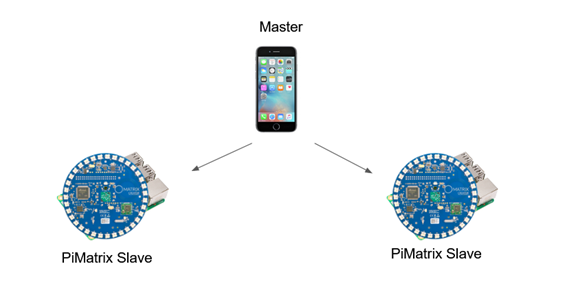
\includegraphics[scale = 1.0]{fig3.1} 
\caption{Overview of System Architecture}
\label{fig}
\end{figure}

Figure 3.1 shows the overall architecture of the proposed system. This design follows the master/slave model, with the PiMatrix devices acting as the slaves and the PiMatrix Control application acting as the master. 

The PiMatrix devices are connected to the PiMatrix Control application by means of tethering themselves to the mobile device’s personal hotspot. In this manner, the system can be deployed anywhere without having to connect to a physical router or wireless access point.  

To provide customization in deployment, the system is not limited to any number of PiMatrix devices. This could aid in speaker diarization applications or simply be used to increase the capture field of the microphone array system. The only limitation would be the range of the mobile device’s hotspot. 

\subsection{PiMatrix Device}

\begin{figure}[h]
\centering
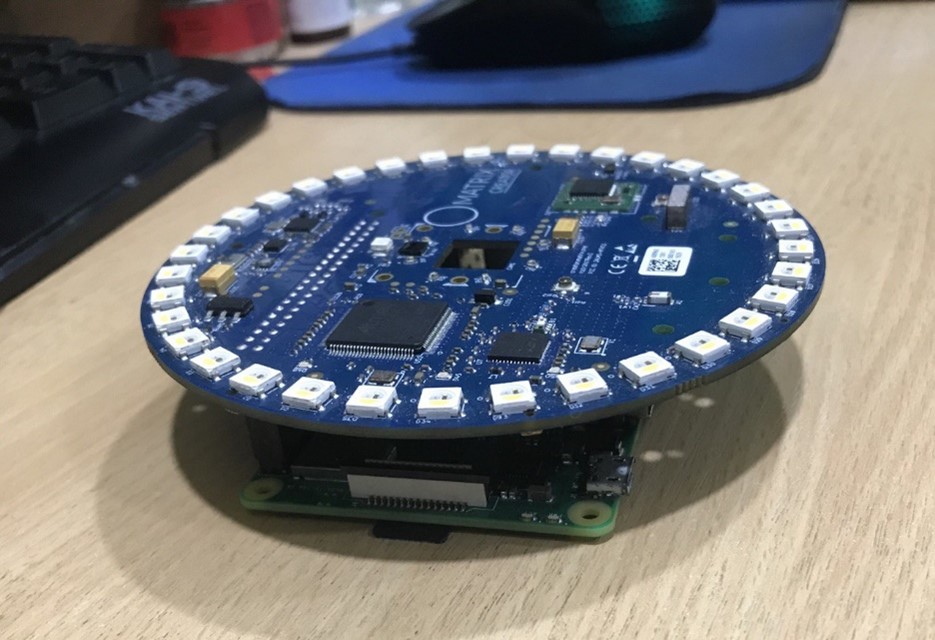
\includegraphics[scale = 1.0]{fig3.2} 
\caption{Assembled PiMatrix Device}
\label{fig}
\end{figure}

As mentioned in the previous section, each PiMatrix device is composed of a MATRIX Creator and a Raspberry Pi connected by their GPIO pins. Each PiMatrix device measures roughly 10.6cm x 10.6cm x 2cm, is lightweight and is highly portable. A standard mobile device power bank with 3.6V and 10000mAh is sufficient to power the device.



\subsubsection{MATRIX Creator}

The MATRIX Creator is an expansion circuit board designed to be used with the Raspberry Pi via the GPIO pins. It features different types of sensors and hardware useful for a variety of applications. For this design, the following components of the MATRIX Creator are used:

	\begin{itemize}
		\item{\textbf{Everloop LED Ring: }}
		it is comprised of 35 LED that are customizable by setting the RGBW values of each individual LED. The LED ring is used to indicate the status of the device to provide visual feedback of the system.
	
		\item{\textbf{Microphone Array: }}
		8 omnidirectional microphones attached to the edge of the device form the circular microphone array of the MATRIX Creator. 
	
		
	\end{itemize}

\subsubsection{Microphone Array}

\begin{figure}[h]
\centering
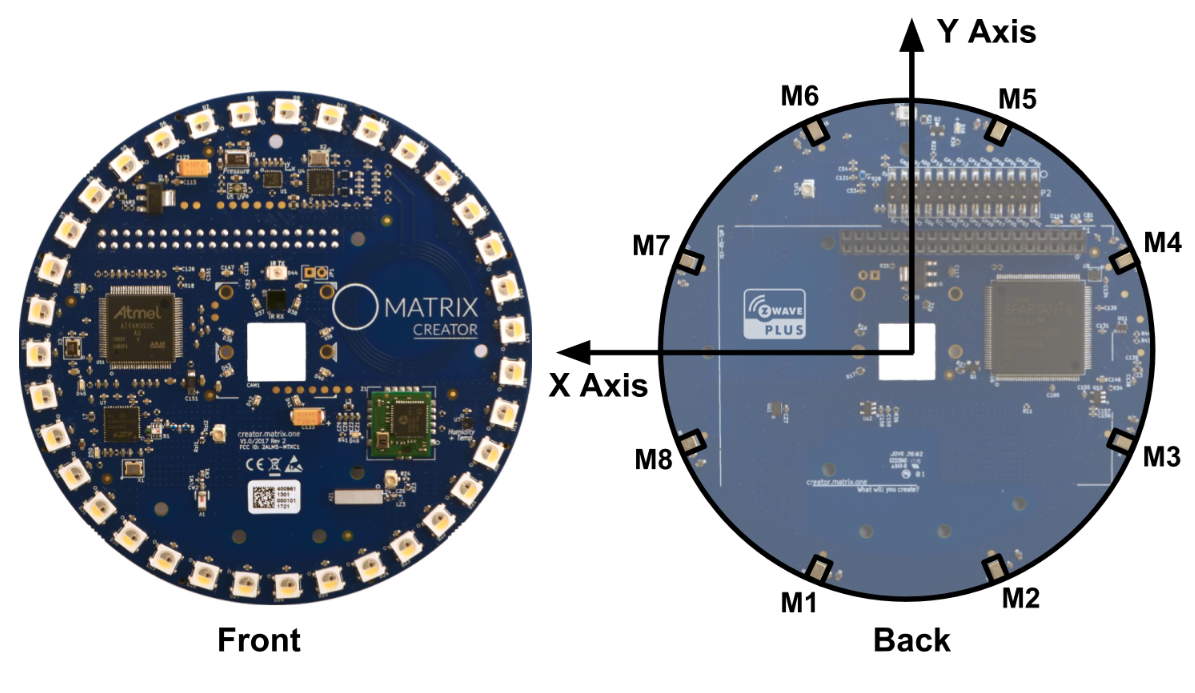
\includegraphics[scale = 0.4]{fig3.3} 
\caption{Diagram of MATRIX Creator Microphone Array}
\label{fig}
\end{figure}

The microphone array consists of 8 omnidirectional MEMS microphones. Figure 3.3 shows the position of the microphones attached to the back of the device. 

The microphones are connected via the Serial Peripheral Interface (SPI) which is a standard for synchronous serial communication over short distances\cite{27}. A master clock is used to control all 8 of the microphones which act as slaves. Data is then transferred during the rising or falling edge of the clock. This ensures that all samples taken from the microphone array are already synchronized. 



\begin{table}[]
\begin{center}
\begin{tabular}{|l|l|l|l|}
\hline
\textbf{Microphone} & \textbf{Ch} & \textbf{X position} & \textbf{Y position} \\ \hline
M1                  & 1           & 20.0908795          & -48.5036755         \\ \hline
M2                  & 2           & -20.0908795         & -48.5036755         \\ \hline
M3                  & 3           & -48.5036755         & -20.0908795         \\ \hline
M4                  & 4           & -48.5036755         & 20.0908795          \\ \hline
M5                  & 5           & -20.0908795         & 48.5036755          \\ \hline
M6                  & 6           & 20.0908795          & 48.5036755          \\ \hline
M7                  & 7           & 48.5036755          & 20.0908795          \\ \hline
M8                  & 8           & 48.5036755          & -20.0908795         \\ \hline
\end{tabular}
\label{tab:tablelabel}
\caption{MATRIX Creator Microphone Channels and Positions}
\end{center}
\end{table}

The microphones are designed to be used with the Advanced Linux Sound Architecture (ALSA) framework. This framework provides an easy application programming interface to access the individual microphones of the MATRIX Creator. Each microphone can be accessed by specifying its channel as shown in Table 3.1. 

The exact angles of the microphones about the X-Y plane is also shown. This could be useful in the development and research of various beamforming and direction-of-arrival applications. A full detailed description of the MEMS microphones used are available in Appendix B.

\subsubsection{Raspberry Pi 3B+}

The Raspberry Pi 3B+ is a single-board computer developed by the Raspberry Pi Foundation. It is a popular tool used for prototyping due to its low cost and portability. It runs the Raspbian operating system which is a Debian-based Linux distribution. 

The Raspberry Pi 3B+ features a 1.4 GHz quad core processor which can safely provide most of the processing power that this system requires. The Raspberry Pi 3B+ also features both WiFi and Bluetooth which are important for wireless communication.

\subsection{PiMatrix Control Mobile Application}

Mobile devices have become widely used in most of the world. Furthermore, most modern mobile devices provide the option to setup a personal wi-fi hotspot. Due to the advantages of portability and the ease of setting up an ad-hoc wireless network, it is determined that a mobile application running on these devices is the most efficient way to control the PiMatrix devices. 

To speed up development and testing, the PiMatrix Control mobile application shall be developed with the cross-platform mobile development framework, Flutter\cite{26}.  

The PiMatrix Control mobile application can be run on any device that supports iOS or Android operating system. The application provides a simple user interface to access the various functions of the PiMatrix device.   

The PiMatrix Control mobile application shall have the following functions:

	\begin{itemize}
		\item{\textbf{Discover Devices: }}
		the application shall have the ability to discover all PiMatrix devices in the same network.
	
		\item{\textbf{Synchronize Devices: }}
		the application shall be able to perform precision time protocol synchronization with all connect PiMatrix devices.

		\item{\textbf{Multichannel Record: }}
		the application shall be able to start synchronized multi-channel recording on all connected PiMatrix devices.

		\item{\textbf{Synchronized Voice Activity Detection: }}
		the application shall be able to start synchronized recording with voice activity detection on all connected PiMatrix devices.

		\item{\textbf{Stop: }}
		the application shall be able to stop all current recordings on the connected PiMatrix devices.

		\item{\textbf{Upload Files: }}
		the application shall be able to control all PiMatrix devices to upload all current recordings to a cloud server.
	
		
	\end{itemize}

\section{Proposed Functional Requirements}

This section describes the functionalities provided by the proposed microphone array system to aid in further research and development for future microphone array applications. 

\subsection{Hot Word Detection}

As the PiMatrix device operates in headless mode without any form of hardware peripherals to control its operation, a hands-free method of controlling the PiMatrix device is needed. For this system, we utilize the microphone array of the MATRIX Creator to control the device with voice commands.

To prevent unnecessary power consumption and usage of computational resources\cite{18}, a hot word detection system is implemented to start the PiMatrix firmware. The system switches off all unused capabilities of the PiMatrix device such as wi-fi and HDMI to reduce the energy consumption of the system. It then continuously listens at regular intervals for the chosen hot word. If the hot word is detected, the detection system then runs the PiMatrix firmware.

\subsection{Network Device Discovery}

To aid flexibility in deployment, the proposed system is able to discover any new devices that join the network in real-time. The mobile application lets users see all devices that are currently connected to the network. 

The PiMatrix Control mobile application would first send a broadcast message to discover all devices on the network, and upon detection of a PiMatrix device, would initiate a handshake protocol. Then it would establish Transmission Control Protocol (TCP) connections with the devices to facilitate communication. 

\subsection{Network Synchronization}

As described in chapter 2.2, network synchronization is crucial for processing different sources of audio information. Ideally, all PiMatrix devices in the network are sample synchronous, which means that all devices have no deviation in the starting and ending time of their samples. Since the PiMatrix devices are recording at a sample rate of 16kHz, each sample would last 62.5 microseconds. 

Two sources of synchronization error are possible in the current architecture:

	\begin{itemize}
		\item{\textbf{Local System Time: }}
		this is the discrepancy between different system clocks among the different PiMatrix devices. 
	
		\item{\textbf{Network Transmission Delay: }}
		this is the delay when sending TCP packets from the master application to the slave devices. 
	
		
	\end{itemize}

\begin{figure}[h]
\centering
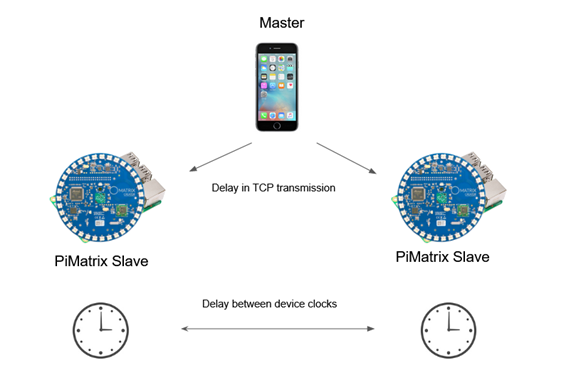
\includegraphics[scale = 1.0]{fig3.4} 
\caption{Diagram of sources of Network Delay}
\label{fig}
\end{figure}

Figure 3.4 above shows the application of synchronization protocols to ensure synchronized recording among devices. Each device’s delay offset from the master mobile device is calculated. The master device then sends a command to start recording at a 1 second off the current time minus each device’s offset. Through this design, each device will start recording at the same time.

\subsubsection{Network Time Protocol}

As the Raspberry Pi does not have a hardware clock built into it, the Raspbian Operating System mimics a clock by saving the software clock time on shutdown and then reloading that time upon reboot. Raspbian tries to get the accurate time by implementing a daemon that acts as a Simple Network Time Protocol (SNTP) client and adjusting its own software clock\cite{28}. 

However, since the implementation of SNTP is relatively simple and only queries time from one remote server. There could be deviation between the clocks of different PiMatrix devices. 

As described in chapter 2, NTP is suitable to be used to synchronize clocks to within tens of milliseconds over the public internet and is thus used for synchronizing the local system time of the various PiMatrix devices instead of the built-in SNTP daemon\cite{14}. 

\subsubsection{Precision Time Protocol}

As NTP is only able to provide millisecond accuracy, PTP is required for a microsecond precision synchronization. The mobile device acts as the master clock in this configuration and exchanges synchronization packets with the slave device. The offset is then calculated as described in chapter 2.2.2. The offset of that device is then saved on the master. This process is repeated among all PiMatrix devices in the network. This offset is then used to counteract the delay incurred over wireless network.

\subsection{Synchronized Multichannel Recording}

To minimize the number of audio files to process, each device shall save the data from the 8 individual microphones into one uncompressing wave file. The individual audio files are separated via the channels as shown in table 3.1, Audio editing software that are able to read wave files will be able to then deconstruct the wave file into their separate channels for individual processing if required. 

Although a sampling rate of 8kHz would be sufficient for most speech related applications\cite{44}, the system may require audio data outside the range of the human voice for certain specialized applications. Thus, for an optimal tradeoff between file size and recording fidelity, a sample rate of 16kHz is used in this system. 

To ensure that all recordings among the various PiMatrix devices begin at the same time, the PiMatrix Control mobile application appends a “time to start” header with each command. The slave PiMatrix devices will then perform the command after a delay determined by the “time to start” header. This “time to start” header is determined by the precision time protocol as described in the previous section.

\subsection{Synchronized Voice Activity Detection}

In this system, all connected devices in a network must capture audio data when sound is detected anywhere in a room. This is because all audio information could contribute to the accuracy of various speech processing algorithms such as acoustic source localization. These algorithms could use the reduced signal of PiMatrix devices further from the sound source to calculate phase of the signal or use the phased version of the same signal to calculate the impulse response of the room\cite{29}. 

\begin{figure}[h]
\centering
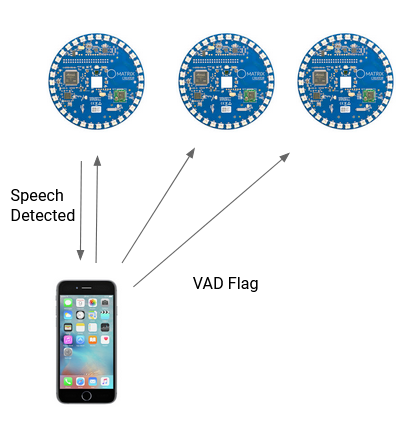
\includegraphics[scale = 1.0]{fig3.5} 
\caption{Overview of Synchronized Voice Activity Detection}
\label{fig}
\end{figure}

Figure 3.5 shows the process of synchronizing voice activity detection among all devices. Whenever voice activity is detected by any of the devices, it sends a signal to the master PiMatrix Control application. The master device then sends a flag to all connected devices while considering the offset delay of each device with the master. When the slave devices receive this flag, it signals them to being capturing audio data. During this process, whenever any of the devices continues to detect spoken signals, this process is then repeated. All devices only stop recording after a certain duration of not receiving any flag, thus all devices will also stop capturing audio data at the same time. This ensures that the length of audio data captured is consistent among all devices.  

\subsection{Beamforming and Direction of Arrival}

As described in chapter 2.2.1 and 2.2.2, beamforming used together with direction of arrival can increase the signal strength of the audio especially in dynamic situations where the position of the speaker is not fixed\cite{9}.

Due to the microphones in the hardware being omnidirectional, there is no method to physically steer the microphones in the direction of the speaker. To simulate the steering of the microphones, recorded audio is converted to an array of 8 channels as shown in table 3.1.

By feeding the data into the MUSIC algorithm, we can estimate the direction of arrival that the data is coming from\cite{11}. Then, to simulate steering the microphones, we can increase the amplitude of the digital audio data as a virtual gain increase. Then to increase the signal to noise ratio, the signals of the microphones in the opposite direction have their amplitude reduced.    

\subsection{Uploading of Audio Data}

Although the recordings are saved locally on the SD card storage of the PiMatrix device, having to repeat the process of removing the SD card and extracting the audio data files is time-consuming. Therefore, this architecture proposes a method to easily upload the files to a storage server. 

The PiMatrix devices can tether to the master mobile device to connect to the internet and upload their files to a cloud storage server. The theoretical maximum transfer speed that the devices can upload their files are determined by the following factors:

	\begin{itemize}
		\item{\textbf{Raspberry Pi Wi-fi speed: }}
		the speed of the WiFi card, which can reach net throughputs of up to 72.2Mbps\cite{30}.
	
		\item{\textbf{Mobile device Wi-fi speed: }}
		the speed of the WiFi system on the mobile device which can vary depending on the device used.

		\item{\textbf{Cellular Network Upload Speed: }}
		the upload speed of the device’s cellular network which is normally controlled by the user’s telecommunications provider company. 
	
		
	\end{itemize}

Therefore, the upload speed is given by the formula:

\begin{equation} \label{eq:1}
    \min{(RaspberryPiWifiSpeed, MobileDeviceWifiSpeed, CellularNetworkUploadSpeed)}
\end{equation}


\subsection{Summary of Design}

In this chapter, the main features of the proposed microphone array system are described, including the system’s hardware, software, and functional requirements. The proposed microphone array system has potential to meet the objectives of the project due to the following factors:

	\begin{itemize}
		\item{\textbf{Accuracy: }}
		by utilizing both Network Time Protocol and Precision Time Protocol, the system will be able to achieve clock accuracy in the sub-microsecond range. Furthermore, a 16kHz sampling rate will allow all significant audio data to be captured and used for further processing. 
	
		\item{\textbf{Portability: }}
		the PiMatrix device used is small and easily portable. Furthermore, any number of PiMatrix devices can be used in this system architecture. The PiMatrix Control mobile application is also able to be run on any mobile device.

		\item{\textbf{Low Power: }}
		each PiMatrix device can be powered by a standard commercial mobile device power bank. By utilizing hot word detection, the battery life of the power bank can be further extended for longer operation.
	
		
	\end{itemize}

\chapter{Implementation of Microphone Array System}

In this chapter, a detailed description of the software running on both the PiMatrix device and the PiMatrix Control mobile application is elaborated. 
This chapter also further describes the implementation of the functional requirements of the proposed system.


\section{Code Repository Overview}

The source code for this project can be found on the following Github Repository:\linebreak

\textit{https://github.com/zuroh/PiMatrix\_System/Mobile\_Version}



	\begin{itemize}
		\item{\textbf{PiMatrix: }}
		contains all the source code to be run on the PiMatrix devices.
		\item{\textbf{PiMatrix\_Control\_App: }}
		contains all the source code required to build the mobile application. 

	
		
	\end{itemize}

\section{PiMatrix Device Firmware}

The firmware for the PiMatrix device was developed in Python 3 due to the amount of useful Python libraries relevant to this project. The \textit{PiMatrix} folder contains the following:

	\begin{itemize}
		\item{\textbf{/pimatrix\_firmware.py: }}
		this is the main source code of the PiMatrix device firmware. This program is called upon the hot word being detected as defined in \textit{hotword\_boot.py}.
		\item{\textbf{/Multirec.py: }}
		contains the module for multichannel synchronized recording.
		\item{\textbf{/Tcp\_sync.pyp: }}
		contains the module to synchronize with a master device over TCP using PTP.
		\item{\textbf{/Upload.py: }}
		contains the module to upload files to a specific folder in google drive.
		\item{\textbf{/Voice\_activity\_detection.pyp: }}
		contains the module that runs the synchronized voice activity detection function. 
		\item{\textbf{/DOA/beamformer.py: }}
		contains the module that estimates direction of arrival and applies beamforming to the incoming signals.
		\item{\textbf{/mycreds.txt: }}
		contains the credentials file used to request an access token to authenticate to Google drive. 
		\item{\textbf{/client\_secrets.json: }}
		contains the access token that allows access to Google drive. 
		\item{\textbf{/Wakeword/Snowboy/wakeword.py: }}
		this program is auto run on PiMatrix boot up. It contains the main logic code for the hot word detection.
		\item{\textbf{/Snowboy/snowboydecoder.py: }}
		a wrapper program for easy usage of Snowboy’s functionalities.
		\item{\textbf{/Snowboy/snowboydetect.py: }}
		this library takes in a hot word model and audio data and returns if the hot word is detected or not.
		\item{\textbf{/Snowboy/Hello\_Matrix.pmdl: }}
		a speech model generated by Snowboy’s web interface. This model lets the decoder detect “Hello Matrix” as a hot word.

		
	\end{itemize}

As each functionality is kept in a separate file, the implementation is modular in nature thus easing development and debugging. These modules can also be easily removed or extended into the system. 

\subsection{Libraries Used}

This section provides a brief description of all the libraries used in the development of the PiMatrix device firmware.

	\begin{itemize}
		\item{\textbf{PyAudio\cite{31}: }}
		a python library that provides bindings for PortAudio.
		\item{\textbf{webrtcVAD\cite{32}: }}
		a python library that provides bindings for the popular WebRTCVAD.
		\item{\textbf{pause\cite{33}: }}
		a python library that allows program execution to halt for a given number of times up to a millisecond precision.
		\item{\textbf{pydrive\cite{34}: }}
		a python library for easy interfacing with Google Drive.
		\item{\textbf{matrix\_lite\cite{35}: }}
		a Python library designed to be able to access all the hardware and sensor data from the MATRIX Creator.  
		\item{\textbf{collections\cite{36}: }}
		a library of data structures, the deque data structure is used in this project. 
		\item{\textbf{Snowboy\cite{37}: }}
		a hot word detection engine that is able to detect chosen hot words. 
		\item{\textbf{ntp\cite{28}: }}
		a Linux implementation of the Network Time Protocol. This package allows the Linux system to act as either an NTP server or NTP client. 

		
	\end{itemize}

\subsection{PiMatrix Firmware Functions}

The firmware code is a multi-threaded python application that runs the main functionality of the PiMatrix devices. The following functions are implemented in \textit{PiMatrix\_firmware.py}:

	\begin{itemize}
		\item{\textbf{\_\_init\_\_: }}
		entry point of the program.
		\item{\textbf{initialize\_threads: }}
		function to initialize all worker threads that are needed during program run-time.
		\item{\textbf{udpBroadcastReceiver: }}
		client function that responds to handshake messages by the master application.
		\item{\textbf{tcpReceiver: }}
		function that waits for commands being sent from the master application.
		\item{\textbf{/tcpSync/tcpSlave: }}
		function that facilitates the precision time protocol synchronization process.  
		\item{\textbf{/voice\_activity\_detection/vad\_record: }}
		function that initiates synchronized VAD recording mode on the PiMatrix device.
		\item{\textbf{/multirec/record2disk: }}
		function that initiates normal synchronized multichannel recording on the PiMatrix device.
		\item{\textbf{/DOA/beamform: }}
		function that takes in audio data, estimates the direction of arrival, and then virtually steers the microphones toward the source signal. 
		\item{\textbf{/upload/uploadFile: }}
		function that uploads all recordings in the current session to a specified cloud storage.

		
	\end{itemize}



\begin{table}[]
\begin{center}
\begin{tabular}{|l|l|l|l|}
\hline
\textbf{LED}     & \textbf{UI Action}                                         & \textbf{Status} & \textbf{State}                                                           \\ \hline
Single Turquoise &                                                            & Idle            & Waiting for Wakeword                                                     \\ \hline
Flash Red        &                                                            & Idle            & Searching for WiFi                                                       \\ \hline
5 Gold           &                                                            & Idle            & Discovered WiFi                                                          \\ \hline
5 Green          & Discover                                                   & Idle            & Discovered Network                                                       \\ \hline
Rotating Blue    & Sync Device                                                & Idle(Sync)      & Synchronizing to Master                                                  \\ \hline
7 Turquoise      & Record                                                     & Recording       & Multichannel Recording                                                   \\ \hline
3 Pink           &                                                            & Recording       & \begin{tabular}[c]{@{}l@{}}Detected \\ Direction of Arrival\end{tabular} \\ \hline
5 Green Flash    & \begin{tabular}[c]{@{}l@{}}Synchronized\\ VAD\end{tabular} & VAD             & Detected Voice Activity                                                  \\ \hline
5 Blue           & Stop Record                                                & Idle            & Audio Saved                                                              \\ \hline
5 Purple         & Upload Files                                               & Upload          & Uploading to Cloud Drive                                                 \\ \hline
5 Blue           & Upload Files                                               & Upload          & Uploading Success                                                        \\ \hline
\end{tabular}
\label{tab:tablelabel}
\caption{Summary of Device States and LED feedback}
\end{center}
\end{table}

To provide easy visual feedback, the firmware program uses the MATRIX Creator’s LED rings to indicate its current state. Table 4.1 shows the indicative LED along with the device state. 

\section{PiMatrix Control Mobile Application}

Due to the advantages discussed in chapter 2.7.3, the mobile application is written in Dart with the Flutter framework. The following files are found in the \textit{FYP\_flutter\_app folder}:

	\begin{itemize}
		\item{\textbf{/build: }}
		contains all required dart build files and configuration settings.
	
		\item{\textbf{/android: }}
		contains all required build files and configuration settings for Android Studio.

		\item{\textbf{/ios: }}
		contains all required build files and configuration settings for Xcode.
		\item{\textbf{/lib: }}
		contains the main source code of the application.
	
		
	\end{itemize}

To simplify development, the state management Bloc is used to separate the presentation from the business logic\cite{38}. In this application, all business logic code can be found in \textit{/lib/logic.dart} and all presentation code can be found in \textit{/lib/main.dart}.

\begin{figure}[h]
\centering

\includegraphics[scale = 0.7]{fig4.1} 
\caption{Bloc Architecture}
\label{fig}
\end{figure}

\textit{Bloc} works by implementing a data structure that provides a state stream between the presentation layer and business logic. Whenever any data is changed in the business logic or events are called from the presentation layer, the stream will notify the other party accordingly. 

The following functions are defined in \textit{/lib/logic.dart}:

	\begin{itemize}
		\item{\textbf{discoverDevices: }}
		function to initiate network device discovery. 
	
		\item{\textbf{tabulateDevices: }}
		function to update all connected devices and their states to the user interface.

		\item{\textbf{syncDevicesTCP: }}
		function to being the precision time protocol synchronization.

		\item{\textbf{sendCommand: }}
		function that sends commands to all connected PiMatrix devices based on user input.

		\item{\textbf{vadUDP: }}
		function that waits for messages while in VAD mode.

		\item{\textbf{disconnectAll: }}
		function to remove all connected devices from the current network.
	
		
	\end{itemize}



\section{Implementation of Functional Requirements}

In this section, the detailed implementation of each of the proposed functional requirements of the system are discussed.

\subsection{Hot Word Detection}

In this project, Snowboy hot word detection engine was used due to the following reasons:

	\begin{itemize}
		\item{\textbf{Customizability: }}
		Snowboy can create customized speech models generated from user submitted recordings to act as the hot word in the system.
	
		\item{\textbf{Resouce Consumption: }}
		Snowboy is more computationally efficient than running an Automatic Speech Recognition system to detect for hot words. On most Raspberry Pi CPU chips, Snowboy takes only about 5-10\% of RAM usage\cite{39}. 
	\end{itemize}

\begin{figure}[h]
\centering
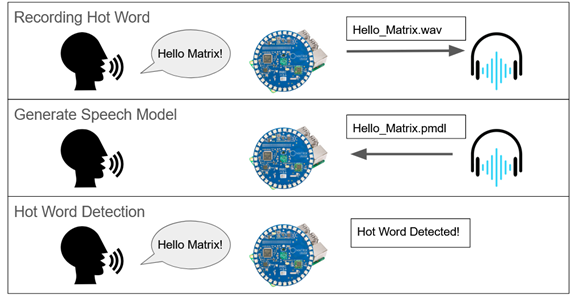
\includegraphics[scale = 1.0]{fig4.2} 
\caption{Diagram of Snowboy Usage}
\label{fig}
\end{figure}

To use Snowboy, a personalized hot word model must first be created. The chosen hot word was recorded on the MATRIX Creator’s microphones; the hot word used for this system was “Hello Matrix”. The recordings were then uploaded to Snowboy’s web interface to generate the personalized model. 

The generated model is then fed to Snowboy’s decoder program, a simple ring buffer is then used by the decoder to assess if the hot word was detected every 0.3 seconds. Upon detection of the hot word, the program then starts the PiMatrix firmware script and enables the WiFi of the PiMatrix device. 

To provide a fully hands-free operation of the microphone array system, the Snowboy hot word detector is configured to automatically run on boot. The Raspberry Pi autostart utility is used to open a LXTerminal and run the script upon device boot to the Raspberry Pi’s desktop. The configurations of the Raspberry Pi’s autostart function can be edited in the textit{~/.config/lxsession/LXDE-pi/autostart} file.

\subsection{Network Device Discovery}

Figure above shows the stages of the device discovery process. Before initiating the protocol, the desired WiFi network credentials should be stored in \textit{/etc/wpa\_supplicant/wpa\_supplicant.conf} file of the PiMatrix device.

Step 1: all activated PiMatrix devices are searching for the mobile device’s personal mobile hotspot. After devices are connected to the mobile device’s personal hotspot, the user can then select “Discover Devices” on the mobile application to initiate the discovery protocol.

Step 2: after selecting the “discover devices” option, the mobile application sends a UDP broadcast message to all devices in the same network with a hard-coded string.

Step 3: upon receiving the message, the individual PiMatrix devices check the string, and if it matches, it sends a hard-coded reply and its own hostname. 

Step 4: the mobile application first checks to see if the reply string is correct, then it checks to see if the device is not currently connected to the mobile application. If both these conditions are true, the mobile application establishes two TCP connections with the device. 

	\begin{itemize}
		\item{The first TCP connection is used to deliver commands from the mobile applications to the PiMatrix devices.}

		\item{The second TCP connection is used to send synchronization packets to carry out the synchronization protocol. The process of synchronization will be explained in the next section.}
	\end{itemize}

If the mobile application does not receive any UDP response within 1 second, it assumes that no devices are currently in the network and waits for the user to initiate the discovery protocol again. 


\subsection{Network Synchronization}

Synchronization is performed in two phases. The first phase happens immediately after the PiMatrix device connects to the mobile device’s wireless hotspot. Each PiMatrix performs a Network Time Protocol request via the Linux NTP package. This process is automatic and not controlled by the user.

The second phase begins when the user selects “Sync Devices” on the PiMatrix Control mobile application. The mobile application will iterate through all currently discovered PiMatrix devices and perform the precision time protocol with each device by exchanging time-stamped synchronization packets. 

The application then stores the delay between each device and itself in a variable textit{final\_offset}. Then, whenever a command is sent, the application appends a header containing a floating-point value of textit{(1 – device.final\_offset)} to the PiMatrix device. 

Each PiMatrix device then uses the pause library to halt execution for the number of nanoseconds as defined by the header value before it resumes execution. Using this method, each device will start at the exact same time relative to the master device.

\subsection{Synchronized Voice Activity Detection}

The synchronized voice activity detection function is designed such that all connected PiMatrix devices will start recording at the same time whenever any of the devices detect speech activity. Figure 4.3 shows the state transition of the entire system.

\begin{figure}[h]
\centering
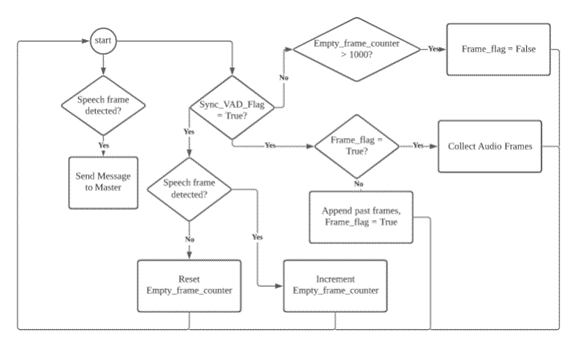
\includegraphics[scale = 1.0]{fig4.3} 
\caption{Synchronized VAD Flowchart}
\label{fig}
\end{figure}

Whenever a single device detects speech activity, it sends a signal to the mobile application. The mobile application then in turn sends a synchronized signal to all devices. This signal sets the textit{sync\_vad\_flag} to true. When this flag is set to true, each PiMatrix device then sets another flag called the textit{frame\_flag} to true. This textit{frame\_flag} signals the device to start collecting audio frames while the textit{sync\_vad\_flag} signals the device that all devices are currently supposed to expect speech activity. 

Whenever a device is recording but no actual spoken frames are detected, it increments a counter called textit{empty\_frame\_counter}. Once this counter exceeds a 1000, the current recording is halted as there is no more speech activity happening in the recording, in this program, 1000 frames of empty audio data corresponds to around 2 seconds of silence. 

A deque that contains the previous 500 audio frames at any given time is stored. Upon the creation of a new VAD chunk, it appends the last 500 audio frames to the start. This ensures that the first utterance in a new VAD chunk is not cut out by accident.

\subsection{Beamforming and Direction of Arrival}

Originally, the doamusic library by Rusell Haley\cite{45} was used, however due to many compatibility issues, it was ultimately not implemented. Therefore, to estimate the direction of arrival, the numpy library was used to convert audio data into a 2D array of 8 channel signals.

A direction of arrival algorithm was implemented to take in a chunk of audio data and return the most likely direction of arrival by calculating the microphone with the most common occurrence of the biggest absolute amplitude. A chunk size of 2048 frames at 16kHz sample rate was fed into the direction of arrival algorithm. This corresponds to about half a second of audio data. 

After returning the directional of arrival, the corresponding LED lights on the Everloop ring are lit up to give a visual indication of the detected direction of arrival. Then, all audio data passing through the given direction of arrival have their amplitudes increased by using numpy to manipulate the array data. In this case, the numpy integer 16 format was used where samples can have an integer value of between -32,768 to 32,767. 

\begin{figure}[h]
\centering
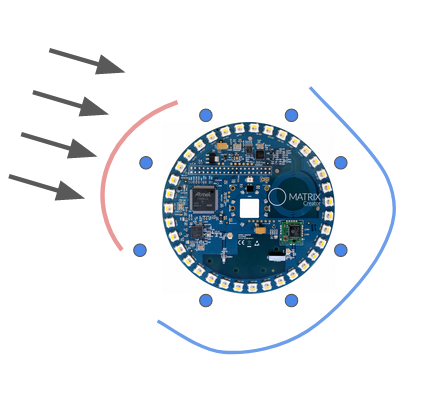
\includegraphics[scale = 1.0]{fig4.4} 
\caption{Diagram of Beamformer}
\label{fig}
\end{figure}

As the microphone array has 8 microphones, 3 microphones will have their signals boosted as indicated by the pink curve in figure 4.4 whereas the remaining 5 will have their signals attenuated to increase the signal to noise ratio. 

\subsection{Uploading of Recordings to Cloud Drive}

The Pydrive library was used to easily provide functionalities to upload local files to Google Drive. The function textit{LoadCredentialsFile} accepts a credentials object which can be created via Google’s OAuth application programming interface. This credentials object represents the current user’s Google Drive account. Once the credentials are loaded, an access token can be generated and the PiMatrix device can upload files directly into the specified google drive directory.

To prevent having to constantly get the access token, this information is saved into the textit{client\_secrets.json} file for easy access each time the firmware is booted up. 

During each network session, all recorded audio files by each PiMatrix device are tracked by an array of file path pointers. Upon selection of “upload file” in the user interface of the mobile application, all currently tracked audio files are uploaded to Google Drive. 



\section{Summary of Implementation}

In this chapter, an explanation for all source code is given and the implementation for certain key functionalities are detailed. This chapter also covers all of the important libraries and packages that are used to implement the microphone array system. 

\chapter{Evaluation of PiMatrix System}

This chapter documents the testing performed on the developed microphone array system to ensure that it meets the objective of performing under real-world conditions. The system was tested on the accuracy of synchronization between devices, power consumption and memory usage. These parameters were chosen with the objective of the project in mind, namely, to develop a microphone array system suitable for usage in a variety of real-world recording environments such as conference meetings. 

\section{Network Synchronization}

This section describes the testing of performance of the two synchronization protocols used in the system. The eight individual microphones that make up each of the microphone arrays are already synchronized, synchronization testing was only done between different microphone arrays. 

\subsection{Testing Method}
\begin{figure}[h]
\centering
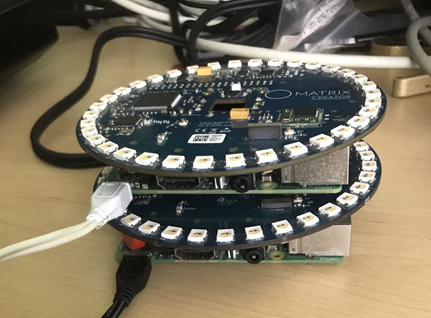
\includegraphics[scale = 1.0]{fig5.1} 
\caption{Stacking of PiMatrix Devices}
\label{fig}
\end{figure}

To test that the devices are sample synchronous when recording, the sound source should ideally arrive at both devices at the same time. However, that is not physically possible due to each device taking up physical space that sound takes time to travel through. Thus, both devices were stacked on top of each other as shown in figure 5.1. A clap is then sounded above the devices to use as the experiment audio data. 

The distance between the microphones of the two devices were measured to be about 2.5 centimeters. Considering the speed of sound travelled in the air, both devices would receive the sound source at approximately 70 microseconds difference. This would be around 1 sample difference given a 16000Hz sampling rate. Therefore, this experiment allows for a margin of error of 1 sample. 

The clap signal was recorded 5 times each for an NTP only synchronized environment, a PTP only synchronized environment and a combination of both synchronization protocols. 


\begin{figure}[h]
\centering
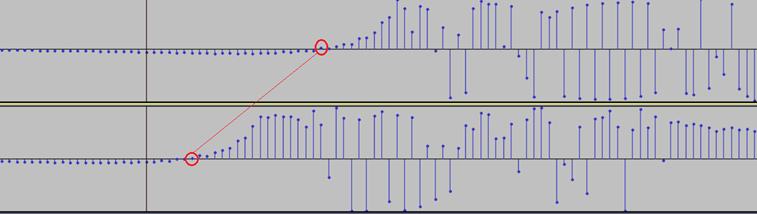
\includegraphics[scale = 1.0]{fig5.2} 
\caption{Sample Difference Measured with Audacity}
\label{fig}
\end{figure}

After the audio samples were recorded, they were analyzed with the audio editing software Audacity. To test the synchronicity of the audio, sample points were chosen by selecting the sample point where the audio switches from the negative amplitude to a positive amplitude. Then the difference in audio samples were calculated. This process was repeated for each recording and their averages calculated. 

\subsection{Testing Results}

This section shows the results of the experiment.

\begin{table}[h]
\begin{center}
\scalebox{0.8}{
\begin{tabular}{|l|l|l|l|l|}
\hline
                                                                         & No Sync & \begin{tabular}[c]{@{}l@{}}Network Time\\ Protocol\end{tabular} & \begin{tabular}[c]{@{}l@{}}Precision Time \\ Protocol\end{tabular} & \begin{tabular}[c]{@{}l@{}}Network + Precision\\ Time Protocol\end{tabular} \\ \hline
\begin{tabular}[c]{@{}l@{}}Avg Sample\\ Difference(samples)\end{tabular} & 527     & 413                                                             & 36                                                                 & 22                                                                          \\ \hline
\end{tabular}}
\label{tab:tablelabel}
\caption{Summary of sample deviation using different synchronization protocols}
\end{center}
\end{table}

\subsection{Evaluation}

The results show a big improvement in sample synchronicity when using precision time protocol as opposed to using network time protocol. Using both network time protocol alongside precision time protocol shows only a modest improvement, however for the purposes of audio synchronization, the improvement is still considered to be useful. Thus, the results show that using both synchronization protocols together is most well suited for the microphone array system. 

It should be noted that none of the synchronization protocols were able to get the system working within one sample difference of each other. This is probably due to the nature of the operating system of the hardware. However, due to the significant improvement in performance when using both PTP and NTP, the obtained results are promising. 

\section{Voice Activity Detection Memory Test}

This section describes the testing performed to determine the effect the VAD has on improving storage memory. All audio samples acquired from VAD testing were re-sequenced together and compared with the original audio recording to ensure that no meaningful spoken audio information was lost.  

\subsection{Testing Method}

To test the VAD system, two microphone array devices were placed one on top of the other like figure 5.1. This was done to ensure that the positions of the microphone array devices did not affect the performance of the VAD as compared to a normal recording. One of the devices was then programmed to record without VAD while the other was programmed to record with VAD. 

Three participants were then placed around the microphone array devices and were told to discuss about a topic of interest to simulate a discussion in a typical conference meeting scenario. 

The collected audio from both devices were then collected and their file sizes compared. Since the VAD splits the recording into separate chunks of audio recordings, the total file size of the chunks was compared against the unbroken complete recording of the discussion.

This process was repeated three more times with each recording timed to be 15 minutes. During the final recording, the participants were told to only speak one word each. Finally, after the recordings were completed, the audio was transcribed, and the number of words were counted. 

\subsection{Testing Results}

This section shows the results of the experiment.

\begin{table}[h]
\begin{center}
\scalebox{0.8}{
\begin{tabular}{|l|l|l|l|l|l|}
\hline
\textbf{}   & \textbf{\begin{tabular}[c]{@{}l@{}}Number of\\ Words\end{tabular}} & \textbf{\begin{tabular}[c]{@{}l@{}l@{}}File Size\\ without\\ VAD(MB)\end{tabular}} & \textbf{\begin{tabular}[c]{@{}l@{}l@{}}File Size\\ with\\ VAD(MB)\end{tabular}} & \textbf{\begin{tabular}[c]{@{}l@{}}Number of \\ VAD Chunks\end{tabular}} & \textbf{\begin{tabular}[c]{@{}l@{}}Memory\\ Improvement\end{tabular}} \\ \hline
Recording 1 & 1524                                                               & 230.4                                                                        & 214.2                                                                     & 35                                                                       & 7\%                                                                   \\ \hline
Recording 2 & 1320                                                               & 230.4                                                                        & 195.7                                                                     & 32                                                                       & 15\%                                                                  \\ \hline
Recording 3 & 1495                                                               & 230.4                                                                        & 215.6                                                                     & 36                                                                       & 7\%                                                                   \\ \hline
Recording 4 & 3                                                                  & 230.4                                                                        & 3                                                                         & 3                                                                        & 99\%                                                                  \\ \hline
\end{tabular}}
\label{tab:tablelabel}
\caption{Comparison of file size between VAD and non VAD recording}
\end{center}
\end{table}


\subsection{Evaluation}

The results show that there is a correlation between the number of words spoken and the performance of the VAD on memory storage saving. This is most likely because the VAD was able to discard more unwanted audio data when there was less speech activity. 

Due to the limited memory storage of the Raspberry Pi, the improvement in memory storage could be a significant factor in the application of the microphone array system. One potential application would be scenarios where vocal speech is not expected for a long period of time. 

\section{Power Consumption Test}

This section describes the testing performed to determine the effect the wake word detection has on power consumption.   

\subsection{Testing Method}


\begin{figure}[h]
\centering
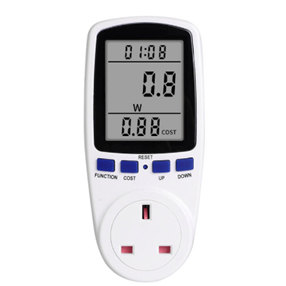
\includegraphics[scale = 1.0]{fig5.3} 
\caption{Wall Power Meter used to measure Power Draw}
\label{fig}
\end{figure}

Device power consumption is most often measured in Amperes(A) thus a power meter was used to detect the current being drawn from the device at any given time. The ampere readings of the PiMatrix device in “passive listening” mode and “active” mode were recorded and measured. This process was repeated 5 times to ensure a consistent result to account for any abnormalities.

\subsection{Testing Results}

This section shows the results of the experiment.


\begin{figure}[h]
\centering
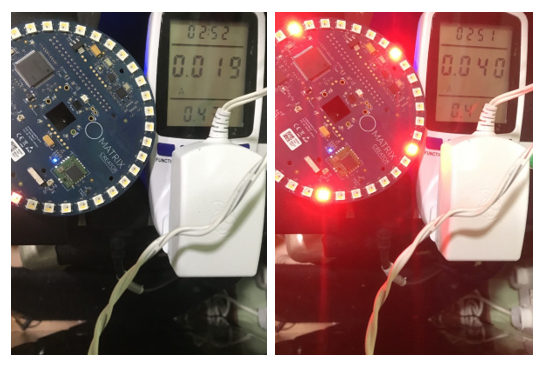
\includegraphics[scale = 1.0]{fig5.4} 
\caption{Power draw of PiMatrix in "passive" mode and "active" mode}
\label{fig}
\end{figure}

\begin{table}[h]
\begin{center}
\begin{tabular}{|l|l|l|}
\hline
              & Passive Listening Mode & Active Mode \\ \hline
Power Draw(A) & 0.019                  & 0.040       \\ \hline
\end{tabular}
\label{tab:tablelabel}
\caption{Average power draw of PiMatrix in "passive" mode and "active" mode}
\end{center}
\end{table}

\subsection{Evaluation}

The results show that the “passive listening” mode can reduce power consumption by about half as compared to its “active” mode. Given a typical power bank with 10000mAh capacity, the battery can last up to 526 hours with the device in “passive listening” mode and 250 hours in its “active” mode. This ensures that the PiMatrix device can be used for long periods while still maintaining its portability in deployment.

\section{Summary of Testing}

In this chapter, the main parameters used to develop a portable and customizable microphone array system were tested. The testing results show that the developed system has achieved the main objectives set out in this project.

	\begin{itemize}
		\item{\textbf{Usability: }}
		the proposed system shows good performance of synchronization between devices which will be useful in further developing speech related applications.
	
		\item{\textbf{Low-memory overhead: }}
		the proposed system shows that a significant number of empty ambient noise can be discarded while recording with the VAD enabled. 

		\item{\textbf{Low-power consumption: }}
		the proposed system demonstrates low power consumption both in “passive listening” mode and “active” mode with “passive listening” mode being twice as energy efficient.

	
		
	\end{itemize}

All these factors combined demonstrate the ability for the developed system to be used as a multi-purpose microphone array system suitable for a wide range of real-world applications.

\chapter{Conclusion}


\section{Summary of Achievements}

In this report, a fully wireless, portable, and customizable microphone array system was developed. This includes both the firmware for the PiMatrix device, along with the companion mobile device application. 

Users can deploy the system anywhere without any bulky equipment, only requiring their mobile device and the PiMatrix devices. Users can also choose to record with any number of PiMatrix devices. 

The developed system can also be left running without much user supervision as the user would only need to wake the device by speaking the chosen wake word. Users can also leave the devices running in normal recording mode or VAD recording mode to only record spoken audio. Finally, users can easily transfer the files to a cloud server via the upload functionality without using any physical drives. 

The usage of an iterative approach helped to streamline the development process. At each stage of iteration, a clear objective was chosen. After completing this objective, the flaws of the first iteration are reviewed and worked on while adding new objectives and functionalities for the next iteration. 


\section{Problems Encountered}

The following section details some of the problems faced during the development of this system as well as the potential reasons and solutions to these issues. 

\subsection{Unpredictable Network Time Protocol Sync}

When the system begins the network time protocol, the time taken to adjust the Raspberry Pi’s system clock is not constant and could last anywhere from between 30 seconds to 2 minutes. 

As I could not figure out how to get the Raspberry Pi to consistently pool the NTP servers at a fixed rate, a system pause was programmed into the starting of the PiMatrix firmware to allow for enough time to let the device synchronize with the NTP servers. 

A possible solution would be to install a hardware clock into the PiMatrix device and save the time upon system shutdown. This way, the PiMatrix device would not lose the synchronized time upon reboot.

\subsection{Unpredictable Detection of Mobile Hotspot}

The Raspberry Pi wireless interface is programmed to automatically join any saved networks upon reboot. However, on occasion the device is unable to detect the wireless hotspot of the mobile device. 

Usually this problem resolves itself by rebooting the wireless hotspot on the mobile device. However, this issue could affect the reliability of the microphone array system. 

Alternative communication protocols such as Bluetooth and Zigbee could resolve this issue but more research is needed in determining the suitability of these communication protocols to support all the functional requirements of the system. 

\section{Future Recommendations}

Due to the limited duration and the large scope of this project, many of the potential applications of this system were not fully explored. Future research and development on this project could explore these topics.

\subsection{Cloud Speech Processing Server}

In the current system, the audio recordings produced by the microphone array system are uploaded to Google Drive for storage. However, there is potential to perform signal processing on the audio data on a backend server. This is especially true in cases where the processing must be performed on recordings produced by different devices as each PiMatrix device cannot perform computation on another device’s recordings. 

\subsection{Speech Enhancement Techniques}

As covered in chapter 2, speech enhancement algorithms could greatly improve the quality of speech recorded by the microphone array. By making use of the individual channels of recorded data, signal processing methods such as dereverberation and beamforming could greatly enhance the overall signal.

Furthermore, these pre-processing algorithms could be performed directly on the PiMatrix device itself before sending the processed signal to be used for other applications such as speech recognition. 

\subsection{Development of Smart Security System}

The nature of the microphone array system to perform long periods of unsupervised recording with little power or memory overhead, lends itself well to be used in a smart security system where the PiMatrix is trained to listen for abnormal audio events and perform some relevant action. 

A camera could be attached to the PiMatrix device to take pictures upon audio detection. Direction of arrival (covered in chapter 2) could then be performed on the recorded audio signal to know where to point the camera to.  

\bibliography{bibliography.bib}

\appendix
\addcontentsline{toc}{chapter}{APPENDICES}
\chapter{MATRIX Creator Components}


\begin{figure}[h]
\centering
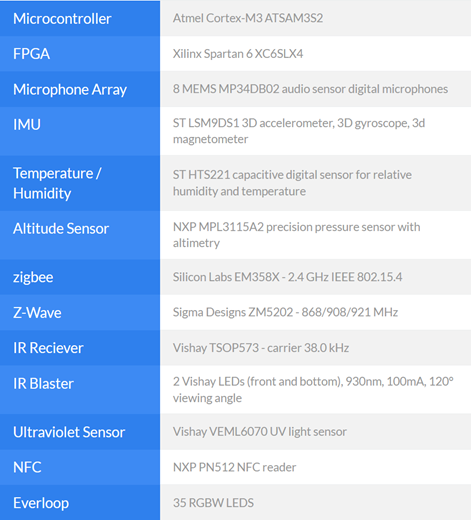
\includegraphics[scale = 1.0]{figa.1} 
\caption{Overview of MATRIX Creator Components}\cite{40}
\label{fig}
\end{figure}

\chapter{MEMS Digital Omnidirectional Microphone}


\begin{figure}[h]
\centering
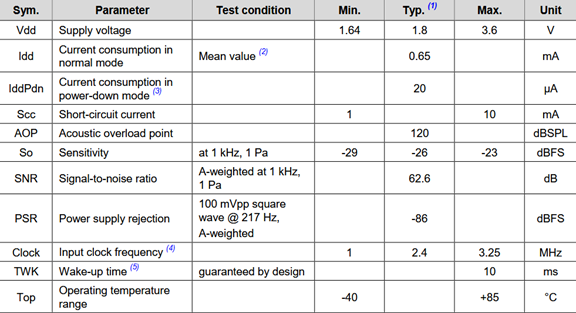
\includegraphics[scale = 1.0]{figb.1} 
\caption{MEMS Omnidirectional Digital Microphone Acoustic and Electrical Features}\cite{41}
\label{fig}
\end{figure}




\end{document}